\documentclass[a5paper]{article}
\usepackage[a5paper, top=8mm, bottom=8mm, left=8mm, right=8mm]{geometry}

\usepackage{polyglossia}
\setdefaultlanguage[babelshorthands=true]{russian}

\usepackage{fontspec}
\setmainfont{FreeSerif}
\newfontfamily{\russianfonttt}[Scale=0.7]{DejaVuSansMono}

\usepackage[font=scriptsize]{caption}

\usepackage{amsmath}
\usepackage{amssymb,amsfonts,textcomp}
\usepackage{color}
\usepackage{array}
\usepackage{hhline}
\usepackage{cite}
\usepackage{textcomp}

\usepackage[hang,multiple]{footmisc}
\renewcommand{\footnotelayout}{\raggedright}

\PassOptionsToPackage{hyphens}{url}\usepackage[xetex,linktocpage=true,plainpages=false,pdfpagelabels=false]{hyperref}
\hypersetup{colorlinks=true, linkcolor=blue, citecolor=blue, filecolor=blue, urlcolor=blue, pdftitle=1, pdfauthor=, pdfsubject=, pdfkeywords=}

\newlength\Colsep
\setlength\Colsep{10pt}

\usepackage{tabu}

\usepackage{graphicx}
\usepackage{indentfirst}
\usepackage{multirow}
\usepackage{subfig}
\usepackage{footnote}
\usepackage{minted}

\newcommand{\todo}[1] {
\begin{center}\textcolor{red}{TODO: #1}\end{center}
}

\newcommand{\attribution}[1] {
    \vspace{-5mm}\begin{flushright}\begin{scriptsize}%\textcolor{gray}
    {\textcopyright\, #1}\end{scriptsize}\end{flushright}
}

\sloppy
\pagestyle{plain}

\title{Лекция 8: Поведенческие шаблоны}
\author{Юрий Литвинов\\\small{yurii.litvinov@gmail.com}}
\date{}

\begin{document}

\maketitle
\thispagestyle{empty}

\section{Паттерн <<Строитель>>}

\subsection{Мотивирующий пример}

Предположим, мы хотим сделать утилиту, которая бы читала текст в некотором формате (допустим, .rtf) и конвертировала бы его в другой формат (например, TeX, .docx, plain text и т.д.). .rtf содержит информацию о структуре текста и его форматировании. Мы не хотим писать несколько разных конвертеров, а хотим считать .rtf один раз и конвертировать его в разные целевые форматы, причём не строя какого-то внутреннего представления (поскольку формат довольно простой и усложнять систему не хотелось бы).

На помощь приходит паттерн <<Строитель>>:

\begin{center}
    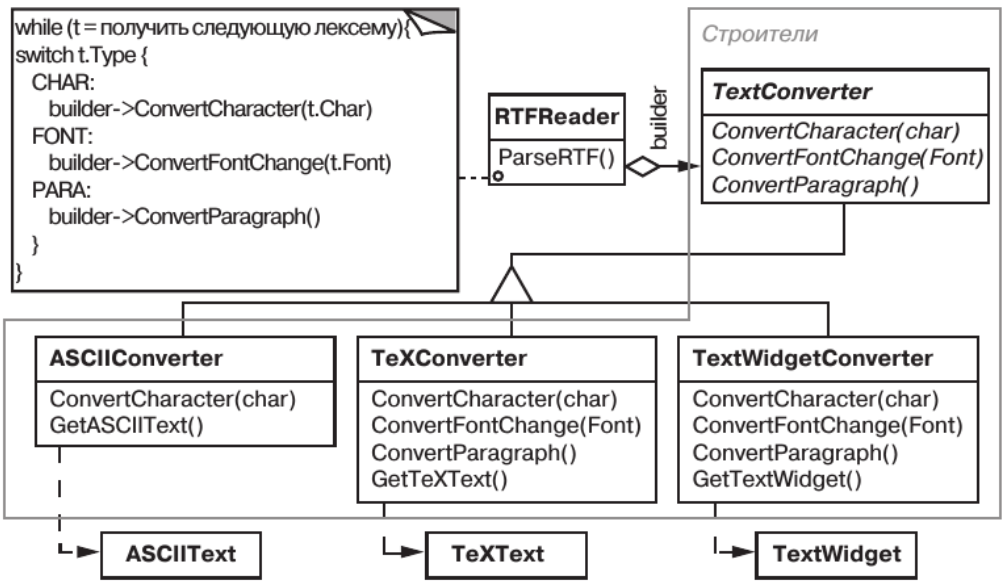
\includegraphics[width=0.9\textwidth]{textConverter.png}
\end{center}

Есть класс RTFReader, который занимается разбором .rtf-документа. Он параметризуется одним из видов конвертеров, каждый из которых принимает элементы документы и что-то с ним делает. Например, ASCIIConverter может просто каждый переданный символ добавлять к строке, а команды форматирования просто игнорировать. Задача RTFReader --- последовательно <<скормить>> весь документ установленному в него конвертеру. Забрать результат потом можно с помощью метода Get-что-то-там у конвертера (они у всех разные).

Теперь, во-первых, процесс конвертации строго детерминирован и управляется централизованно в RTFReader, во-вторых, конвертеры легко менять, поскольку они реализуют один интерфейс и RTFReader-у всё равно, с кем из них работать. И реализовывать конвертеры просто, поскольку им не надо заботиться о разборе документа, и пони получают документ маленькими частями.

\subsection{Строитель (Builder), общая структура}

Эта идея обобщается до паттерна <<Строитель>>:

\begin{center}
    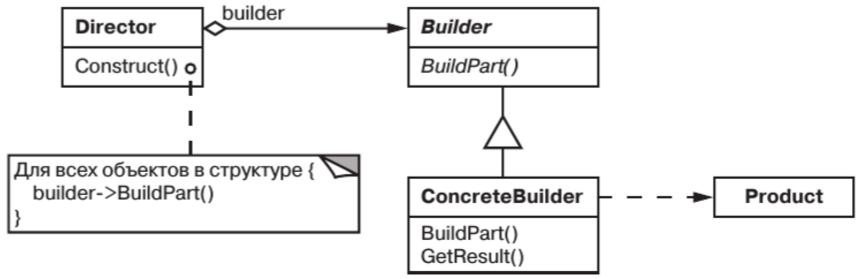
\includegraphics[width=0.8\textwidth]{builder.png}
    \attribution{Э. Гамма и др., Приемы объектно-ориентированного проектирования}
\end{center}

\subsection{Детали реализации}



\section{Паттерн <<Шаблонный метод>>}

\subsection{Мотивирующий пример}

\subsection{Шаблонный метод (Template method), общая структура}

\subsection{Детали реализации}



\section{Паттерн <<Посредник>>}

\subsection{Мотивирующий пример}

\subsection{Посредник (Mediator), общая структура}

\subsection{Детали реализации}



\section{Паттерн <<Команда>>}

\subsection{Мотивирующий пример}

\subsection{Команда (Command), общая структура}

\subsection{Детали реализации}



\section{Паттерн <<Цепочка ответственности>>}

\subsection{Мотивирующий пример}

\subsection{Цепочка ответственности (Chain of Responsibility), общая структура}

\subsection{Детали реализации}



\section{Паттерн <<Наблюдатель>>}

\subsection{Мотивирующий пример}

\subsection{Наблюдатель (Observer), общая структура}

\subsection{Детали реализации}



\section{Паттерн <<Состояние>>}

\subsection{Мотивирующий пример}

\subsection{Состояние (State), общая структура}

\subsection{Детали реализации}



\section{Паттерн <<Посетитель>>}

\subsection{Мотивирующий пример}

\subsection{Посетитель (Visitor), общая структура}

\subsection{Детали реализации}



\section{Паттерн <<Хранитель>>}

\subsection{Мотивирующий пример}

\subsection{Хранитель (Memento), общая структура}

\subsection{Детали реализации}



\section{Паттерн <<Интерпретатор>>}

\subsection{Мотивирующий пример}

\subsection{Интерпретатор (Interpreter), общая структура}

\subsection{Детали реализации}



\section{Паттерн <<Итератор>>}

\subsection{Мотивирующий пример}

\subsection{Итератор (Iterator), общая структура}

\subsection{Детали реализации}

\end{document}